% MATH 6660 -- Homework 2 -- solutions.  Equations numbered for later reference.
% Build: pdflatex hw2_solutions.tex   (twice, for the cross-references)
\documentclass[11pt]{article}
\usepackage[letterpaper,margin=1in]{geometry}
\usepackage[T1]{fontenc}
\usepackage{amsmath,amssymb,amsthm}
\usepackage{booktabs}
\usepackage{graphicx}
\usepackage{caption}
\usepackage{bm}
\usepackage{tikz}
\usetikzlibrary{arrows.meta}
\newcommand{\dx}{\,\mathrm{d}x}
\newcommand{\norm}[1]{\lVert #1\rVert}
\newcommand{\note}[1]{\par\smallskip{\small\textit{Note.}\ #1}\par\smallskip}
\setlength{\parindent}{0pt}

\usepackage{xcolor}
\usepackage[colorlinks=true,linkcolor={blue!45!black},pdfborder={0 0 0}]{hyperref}
\usepackage{pdfcomment}

% ---- hover tooltips on cross-references --------------------------------
% \settip{label}{plain-text summary} registers what pops up on mouse-over;
% \eqr{label} prints (n) as a link AND shows that summary on hover.
\makeatletter
\newcommand{\settip}[2]{\expandafter\gdef\csname femtip@#1\endcsname{#2}}
\newcommand{\gettip}[1]{%
  \ifcsname femtip@#1\endcsname\csname femtip@#1\endcsname\else equation \ref{#1}\fi}
\newcommand{\eqr}[1]{\pdftooltip{\eqref{#1}}{\gettip{#1}}}
\makeatother

% ---- tooltip text for each numbered equation ----
\settip{eq:ode}{Periodic BVP: -u'' + q(x) u = f(x) on (-pi,pi), with u(-pi)=u(pi), u'(-pi)=u'(pi), and q>0}
\settip{eq:mult}{Multiply the ODE by v and integrate: integral of (-u'' + qu) v dx = integral of f v dx}
\settip{eq:parts}{After one integration by parts: integral of (u'v' + quv) dx minus the boundary bracket equals integral of f v}
\settip{eq:bdry}{Boundary bracket = u'(pi)v(pi) - u'(-pi)v(-pi), which vanishes by BC2 together with periodicity of v}
\settip{eq:space}{V = { v : v and v' square integrable on (-pi,pi), and v(-pi) = v(pi) }}
\settip{eq:var}{Variational problem: find u in V with integral of (u'v' + q u v) dx = integral of f v dx for all v in V}
\settip{eq:fem}{CG FEM: find U in Vh with integral of (U'v' + q U v) dx = integral of f v dx for all v in Vh}
\settip{eq:varh}{The exact u tested only against the subspace: integral of (u'v' + q u v) dx = integral of f v dx for all v in Vh}
\settip{eq:go}{Galerkin orthogonality: integral of (e'v' + q e v) dx = 0 for all v in Vh, where e = u - U}
\settip{eq:aform}{Bilinear form a(v,w) = integral over (-pi,pi) of (v'w' + q v w) dx}
\settip{eq:goa}{Galerkin orthogonality restated: a(e,v) = 0 for every v in Vh}
\settip{eq:posdef}{a(v,v) = integral of ( (v')^2 + q v^2 ) dx, which is >= 0 and vanishes only for v identically zero}
\settip{eq:enorm}{Energy norm: ||v||_E = square root of the integral of ( (v')^2 + q v^2 ) dx}

% ---- Problem 2 ----
\settip{eq:mesh}{Uniform mesh: h = 2 pi divided by (M+1), with nodes x j = -pi + j h for j = 0 up to M+1}
\settip{eq:Vh}{Vh = { v in V : v restricted to each element is a linear polynomial }, continuous and periodic}
\settip{eq:hat}{Interior hat phi j: rises from 0 to 1 on the element left of node j, falls back to 0 on the element right of it}
\settip{eq:hat0}{Wrap-around hat phi 0: the right half sits on the first element, the left half sits on the last element}
\settip{eq:span}{Vh = span of phi 0, phi 1, ..., phi M, so the dimension is M+1}
\settip{eq:trial}{Trial function: U = sum over j from 0 to M of xi j times phi j, where xi j is the nodal value of U at node j}
\settip{eq:cg1}{CG(1) method: find U in Vh with integral of (U'v' + q U v) dx = integral of f v dx for all v in Vh}
\settip{eq:system}{Linear system A xi = b of size (M+1) by (M+1)}
\settip{eq:entries}{A i j = integral of (phi i' phi j' + q phi i phi j) dx, and b i = integral of f phi i dx}
\settip{eq:stiff}{Stiffness part: diagonal entries 2 over h, first off-diagonal entries minus 1 over h}

% ---- Problem 3 ----
\settip{eq:opt}{Optimality: the energy norm of u minus U is less than or equal to that of u minus v, for every v in Vh}
\settip{eq:split}{Split u minus v as e plus w, where e = u minus U is the error and w = U minus v lies in Vh}
\settip{eq:expand3}{Expand a(e+w, e+w) = a(e,e) + 2 a(e,w) + a(w,w)}
\settip{eq:pyth}{Pythagoras: the squared energy norm of u minus v equals that of e plus that of w}
\settip{eq:interp}{Interpolation estimates from Lecture 7, for the nodal interpolant}
\settip{eq:enorminterp}{Energy norm of the interpolation error, bounded term by term}
\settip{eq:apriori}{A priori estimate: the energy norm of u minus U is at most C h times the L2 norm of u double prime}

% ---- Problem 4 ----
\settip{eq:dual}{Dual problem: minus phi double prime plus q phi = e, with periodic conditions on phi and phi prime}
\settip{eq:dualvar}{Variational form of the dual problem: a(phi, v) = the L2 inner product of e and v, for all v in V}
\settip{eq:chain}{Chain: the squared L2 norm of e equals a(e, phi minus its interpolant), bounded by the product of two energy norms}
\settip{eq:phibound}{L2 norm of phi is at most the L2 norm of e divided by q min}
\settip{eq:stab}{Stability: L2 norm of phi double prime is at most C S times the L2 norm of e, with C S = 1 + q max over q min}
\settip{eq:l2}{A priori L2 estimate: the L2 norm of u minus U is at most C times h squared times the L2 norm of u double prime}

% ---- Problem 5 ----
\settip{eq:elem}{Element stiffness, q-weighted element mass, and element load on one element}
\settip{eq:wrap}{Local-to-global map: element e connects node e to node (e+1) modulo N, which is the periodic wrap}
\settip{eq:rate}{Observed rate between two consecutive meshes: log of the error ratio over log of the mesh-size ratio}

% ---- Problems 6 and 7 ----
\settip{eq:p6num}{Half-integer numbering k = 0 to 2M+2, with the two Dirichlet ends removed, leaving 2M+1 unknowns}
\settip{eq:p6shape}{Quadratic Lagrange basis on the reference element: vertex, midside, vertex}
\settip{eq:p6Ke}{Element stiffness matrix, equal to one over 3h times the integer matrix with 7, -8, 1 in the first row}
\settip{eq:p6assembled}{The assembled matrix at M = 4, scaled by 3h: the pentadiagonal matrix of Lecture 10}
\settip{eq:p7data}{Check that minus u double prime equals f for the Problem 7 data}

\begin{document}

\begin{center}
  {\large\textbf{MATH 6660 --- Homework 2}}\\[0.2em]
  Hasan
\end{center}
\vspace{0.5em}

% ==================================================================
\section*{Problem 1}

\textbf{Problem.} For the periodic boundary value problem
\begin{equation}\label{eq:ode}
  \textbf{ODE}:\ -u''+q(x)\,u=f(x),
  \qquad
  \textbf{BC1}:\ u(-\pi)=u(\pi),
  \qquad
  \textbf{BC2}:\ u'(-\pi)=u'(\pi),
\end{equation}
with $q>0$ for all $x\in[-\pi,\pi]$, derive a Galerkin orthogonality expression
and deduce from it an appropriate \emph{energy norm}.

\subsection*{Solution}

\textbf{Step 1: variational form.}
Multiply \eqr{eq:ode} by a test function $v$ and integrate over $(-\pi,\pi)$:
\begin{equation}\label{eq:mult}
  \int_{-\pi}^{\pi}\bigl(-u''+q\,u\bigr)v\dx=\int_{-\pi}^{\pi}f\,v\dx .
\end{equation}
Integrate the second-derivative term by parts once:
\begin{equation}\label{eq:parts}
  \int_{-\pi}^{\pi}\bigl(u'v'+q\,u\,v\bigr)\dx
  \;-\;\underbrace{\bigl[\,u'v\,\bigr]_{-\pi}^{\pi}}_{\text{boundary term}}
  \;=\;\int_{-\pi}^{\pi}f\,v\dx .
\end{equation}
The boundary term is
\begin{equation}\label{eq:bdry}
  \bigl[\,u'v\,\bigr]_{-\pi}^{\pi}
   = u'(\pi)\,v(\pi)-u'(-\pi)\,v(-\pi)
   = u'(\pi)\bigl[\,v(\pi)-v(-\pi)\,\bigr]
   = 0 ,
\end{equation}
where \textbf{BC2} was used to replace $u'(-\pi)$ by $u'(\pi)$, and the last
equality holds provided $v$ is periodic. That requirement is what fixes the
space:
\begin{equation}\label{eq:space}
  V=\Bigl\{\,v:\ \int_{-\pi}^{\pi}\bigl(v^{2}+(v')^{2}\bigr)\dx<\infty,
    \ \ v(-\pi)=v(\pi)\,\Bigr\}.
\end{equation}
Dropping \eqr{eq:bdry} from \eqr{eq:parts} gives the variational problem: find
$u\in V$ such that
\begin{equation}\label{eq:var}
  \int_{-\pi}^{\pi}\bigl(u'v'+q\,u\,v\bigr)\dx=\int_{-\pi}^{\pi}f\,v\dx
  \qquad\forall\,v\in V .
\end{equation}

\note{Only \textbf{BC1} is built into $V$ in \eqr{eq:space}; \textbf{BC2} is
\emph{natural}, never imposed on the space. Two points are worth being precise
about. First, BC2 \emph{alone} does not make \eqr{eq:bdry} vanish: it lets the
two endpoint terms be collected into the single factor
$u'(\pi)\bigl[v(\pi)-v(-\pi)\bigr]$, which then vanishes because $v\in V$ is
periodic. It takes both. Second, BC2 is genuinely \emph{recovered} from
\eqr{eq:var}, in two steps. First test with $v$ compactly supported in
$(-\pi,\pi)$: this gives $u''=qu-f$ distributionally, so $u''\in L^{2}$ and
$u\in H^{2}$ --- which is what makes $u'(\pm\pi)$ meaningful and the next step
legal. Now reverse the integration by parts for general $v\in V$:
$\int_{-\pi}^{\pi}\bigl(-u''+qu-f\bigr)v\dx+\bigl[u'v\bigr]_{-\pi}^{\pi}=0$. The
integral vanishes by what was just shown, leaving
$\bigl(u'(\pi)-u'(-\pi)\bigr)v(\pi)=0$; choosing any $v\in V$ with
$v(\pi)\neq0$ forces $u'(-\pi)=u'(\pi)$. Trial and test space coincide.}

\medskip
\textbf{Step 2: the finite element method.}
Choose any finite-dimensional $V_h\subset V$. The FEM is: find $U\in V_h$ such
that
\begin{equation}\label{eq:fem}
  \int_{-\pi}^{\pi}\bigl(U'v'+q\,U\,v\bigr)\dx=\int_{-\pi}^{\pi}f\,v\dx
  \qquad\forall\,v\in V_h .
\end{equation}

\medskip
\textbf{Step 3: subtract.}
Because $V_h\subset V$, the exact solution $u$ satisfies \eqr{eq:var} in
particular for every $v\in V_h$:
\begin{equation}\label{eq:varh}
  \int_{-\pi}^{\pi}\bigl(u'v'+q\,u\,v\bigr)\dx=\int_{-\pi}^{\pi}f\,v\dx
  \qquad\forall\,v\in V_h .
\end{equation}
Subtracting \eqr{eq:fem} from \eqr{eq:varh}, the right-hand sides cancel. With
the error $e:=u-U$,
\begin{equation}\label{eq:go}
  \boxed{\;\int_{-\pi}^{\pi}\bigl(e'v'+q\,e\,v\bigr)\dx=0
         \qquad\forall\,v\in V_h\;}
\end{equation}
which is the Galerkin orthogonality expression for this problem.

\medskip
\textbf{Step 4: read off the energy norm.}
Define the bilinear form appearing on the left of \eqr{eq:var}:
\begin{equation}\label{eq:aform}
  a(v,w):=\int_{-\pi}^{\pi}\bigl(v'w'+q\,v\,w\bigr)\dx .
\end{equation}
Then \eqr{eq:go} reads
\begin{equation}\label{eq:goa}
  a(e,v)=0\qquad\forall\,v\in V_h ,
\end{equation}
i.e.\ the error is orthogonal to the whole subspace \emph{with respect to $a$}.
For that statement to be genuine orthogonality, $a$ must be an inner product on
$V$:

\begin{itemize}\setlength{\itemsep}{2pt}
\item \emph{bilinear} --- each slot is linear, by inspection of \eqr{eq:aform};
\item \emph{symmetric} --- $a(v,w)=a(w,v)$, again by inspection;
\item \emph{positive definite} ---
\begin{equation}\label{eq:posdef}
  a(v,v)=\int_{-\pi}^{\pi}\Bigl[\,(v')^{2}+q\,v^{2}\,\Bigr]\dx\;\ge\;0 ,
\end{equation}
and both terms are non-negative, so $a(v,v)=0$ forces $v'\equiv0$ \emph{and},
since $q>0$, $v\equiv0$.
\end{itemize}

Hence $a$ induces a norm, and it is the appropriate energy norm here:
\begin{equation}\label{eq:enorm}
  \boxed{\;\norm{v}_{E}:=\sqrt{a(v,v)}
    =\left(\int_{-\pi}^{\pi}\Bigl[\,(v')^{2}+q\,v^{2}\,\Bigr]\dx\right)^{1/2}\;}
\end{equation}

\medskip
\textbf{Where $q>0$ is used.} Not decoration. Under periodic conditions,
$v'\equiv0$ only gives $v=\text{const}$, and a constant \emph{is} an element of
$V$ in \eqr{eq:space} --- it is periodic. So $\int(v')^{2}\dx$ alone is a
seminorm, not a norm: it cannot see constants. The term $q\,v^{2}$ in
\eqr{eq:posdef} is exactly what rules them out.

\note{Contrast HW1's Dirichlet problem, where $v(0)=0$ removes the constant for
free and $\int a(x)\,(v')^{2}\dx$ was already a norm on its own.}

\note{\textbf{Standing hypothesis on $q$.} The problem statement gives only
\emph{pointwise} positivity, $q(x)>0$, and that is all \eqr{eq:posdef} needs:
both integrands are non-negative and $q>0$ forces $v\equiv0$. Problems~3
and~4, however, use $q_{\max}=\max q$ and $q_{\min}=\min q>0$, and a uniform
positive lower bound is strictly stronger than pointwise positivity. From here
on assume in addition that $q$ is continuous on the compact interval
$[-\pi,\pi]$; then both extrema are attained and
$0<q_{\min}\le q(x)\le q_{\max}<\infty$. The data of Problem~5 satisfy this,
with $q_{\min}=2-\sqrt2\approx0.586$ at $x=\pi/4$ and $q_{\max}\approx4.25$.}

\clearpage
% ==================================================================
\section*{Problem 2}

\textbf{Problem.} Develop a CG(1) method for \eqr{eq:ode}, clearly stating the
appropriate spaces, trial, test, and basis functions.

\subsection*{Solution}

\textbf{Mesh.} Take the uniform mesh of the hint:
\begin{equation}\label{eq:mesh}
  h=\frac{2\pi}{M+1},\qquad
  x_j=-\pi+j\,h,\quad j=0,1,\dots,M+1,
  \qquad\text{so } x_0=-\pi,\ \ x_{M+1}=\pi .
\end{equation}
The elements are $I_j=[x_{j-1},x_j]$, $j=1,\dots,M+1$ --- so there are $M+1$
elements. Periodicity identifies $x_0\equiv x_{M+1}$, leaving $M+1$
\emph{distinct} nodes rather than $M+2$.

\medskip
\textbf{Spaces.} The continuous space is $V$ from \eqr{eq:space}. The discrete
space is
\begin{equation}\label{eq:Vh}
  V_h=\bigl\{\,v\in V:\ v|_{I_j}\in P_1(I_j),\ \ j=1,\dots,M+1\,\bigr\},
\end{equation}
continuous piecewise linear functions that are also periodic. By construction
$V_h\subset V$, so the method is conforming and Galerkin orthogonality
\eqr{eq:go} applies verbatim.

\note{$\dim V_h=M+1$. A continuous piecewise linear function on $M+1$ elements
carries $M+2$ nodal values $\xi_0,\dots,\xi_{M+1}$, and periodicity forces
$\xi_0=\xi_{M+1}$, removing one. Compare the Dirichlet problem, where
\emph{two} values are removed by prescribing them, leaving $M$. Here one value
is removed by an \emph{identification}, not by prescription.}

\medskip
\textbf{Basis functions.} For the interior nodes $j=1,\dots,M$, the usual hat:
\begin{equation}\label{eq:hat}
  \varphi_j(x)=
  \begin{cases}
    \dfrac{x-x_{j-1}}{h}, & x_{j-1}\le x\le x_j,\\[2ex]
    \dfrac{x_{j+1}-x}{h}, & x_j\le x\le x_{j+1},\\[1.2ex]
    0, & \text{otherwise.}
  \end{cases}
\end{equation}
At the glued node there is one \emph{wrap-around} hat:
\begin{equation}\label{eq:hat0}
  \varphi_0(x)=
  \begin{cases}
    \dfrac{x_1-x}{h}, & x_0\le x\le x_1,\\[2ex]
    \dfrac{x-x_M}{h}, & x_M\le x\le x_{M+1},\\[1.2ex]
    0, & \text{otherwise.}
  \end{cases}
\end{equation}
On the interval $\varphi_0$ looks like two half-hats, one at each end; on the
circle it is a single ordinary hat that the interval happens to cut in two. The
nodal property still holds, $\varphi_i(x_j)=\delta_{ij}$, reading $x_{M+1}$ as
$x_0$. Hence
\begin{equation}\label{eq:span}
  V_h=\operatorname{span}\{\varphi_0,\varphi_1,\dots,\varphi_M\},
  \qquad \dim V_h=M+1 .
\end{equation}

\begin{center}
\begin{minipage}{0.97\linewidth}
\centering
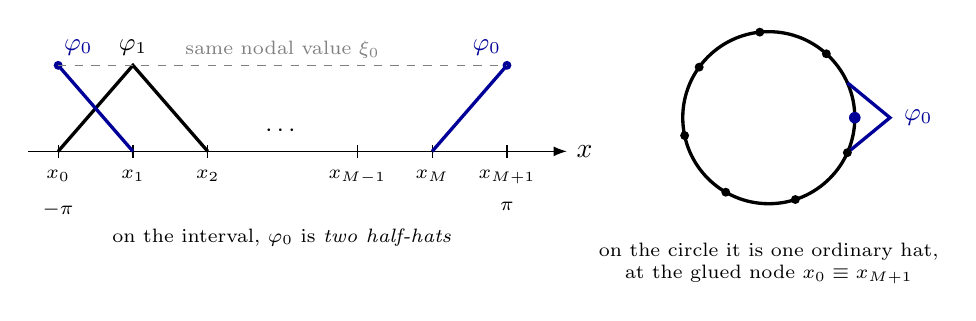
\begin{tikzpicture}[>=Latex,scale=0.95]

% ---------------- left: the interval ----------------
\draw[->] (-0.4,0) -- (6.8,0) node[right] {$x$};
% ticks and labels
\foreach \i/\lab in {0/{x_0},1/{x_1},2/{x_2},4/{x_{M-1}},5/{x_M},6/{x_{M+1}}}{
  \draw (\i,-0.09) -- (\i,0.09);
  \node[below,font=\scriptsize] at (\i,-0.12) {$\lab$};}
\node[font=\small] at (3,0.28) {$\cdots$};
\node[below,font=\scriptsize] at (0,-0.55) {$-\pi$};
\node[below,font=\scriptsize] at (6,-0.55) {$\pi$};
% interior hat phi_1
\draw[very thick] (0,0) -- (1,1.15) -- (2,0);
\node[above,font=\small] at (1,1.15) {$\varphi_1$};
% wrap-around hat phi_0, two halves
\draw[very thick,blue!60!black] (0,1.15) -- (1,0);
\draw[very thick,blue!60!black] (5,0) -- (6,1.15);
\node[above right,font=\small,blue!60!black] at (-0.05,1.15) {$\varphi_0$};
\node[above left,font=\small,blue!60!black]  at (6.05,1.15) {$\varphi_0$};
\fill[blue!60!black] (0,1.15) circle (1.7pt);
\fill[blue!60!black] (6,1.15) circle (1.7pt);
\draw[dashed,gray] (0,1.15) -- (6,1.15);
\node[font=\scriptsize,gray] at (3,1.36) {same nodal value $\xi_0$};
\node[font=\scriptsize,align=center] at (3,-1.15)
     {on the interval, $\varphi_0$ is \emph{two half-hats}};

% ---------------- right: the circle ----------------
\begin{scope}[shift={(9.5,0.45)}]
  \draw[very thick] (0,0) circle (1.15);
  % the hat, drawn outward at angle 0
  \draw[very thick,blue!60!black]
       (24:1.15) -- (1.62,0) -- (-24:1.15);
  \fill[blue!60!black] (0:1.15) circle (2.2pt);
  \node[right,font=\small,blue!60!black] at (1.68,0) {$\varphi_0$};
  % a few other nodes
  \foreach \a in {48,96,144,192,240,288,336}{\fill (\a:1.15) circle (1.7pt);}
  \node[font=\scriptsize,align=center] at (0,-1.95)
       {on the circle it is one ordinary hat,\\
        at the glued node $x_0\equiv x_{M+1}$};
\end{scope}

\end{tikzpicture}
\par\smallskip
{\small The two ends of the interval are the same point of the domain, so the
two half-hats in \eqr{eq:hat0} are two pieces of one basis function and share a
single unknown $\xi_0$. Cutting the circle open to lay it flat is what splits
that hat in half.}
\end{minipage}
\end{center}

\medskip
\textbf{Trial and test functions.} Trial and test space coincide (Galerkin):
\begin{equation}\label{eq:trial}
  \text{trial:}\quad U(x)=\sum_{j=0}^{M}\xi_j\,\varphi_j(x),
  \ \ \xi_j=U(x_j);
  \qquad\qquad
  \text{test:}\quad v=\varphi_i,\ \ i=0,1,\dots,M .
\end{equation}

\medskip
\textbf{The CG(1) method.} Find $U\in V_h$ such that
\begin{equation}\label{eq:cg1}
  \int_{-\pi}^{\pi}\bigl(U'v'+q\,U\,v\bigr)\dx=\int_{-\pi}^{\pi}f\,v\dx
  \qquad\forall\,v\in V_h .
\end{equation}
Substituting \eqr{eq:trial} and taking $v=\varphi_i$ for $i=0,\dots,M$ turns
\eqr{eq:cg1} into
\begin{equation}\label{eq:system}
  \sum_{j=0}^{M}\xi_j
  \int_{-\pi}^{\pi}\bigl(\varphi_i'\varphi_j'+q\,\varphi_i\varphi_j\bigr)\dx
  =\int_{-\pi}^{\pi}f\,\varphi_i\dx ,
  \qquad\text{i.e.}\qquad
  \bm{A}\,\bm{\xi}=\bm{b},
\end{equation}
with
\begin{equation}\label{eq:entries}
  A_{ij}=\int_{-\pi}^{\pi}\bigl(\varphi_i'\varphi_j'+q\,\varphi_i\varphi_j\bigr)\dx ,
  \qquad
  b_i=\int_{-\pi}^{\pi}f\,\varphi_i\dx ,
  \qquad i,j=0,1,\dots,M .
\end{equation}

\medskip
\textbf{Structure of $\bm{A}$.} On the uniform mesh $\varphi_j'=\pm1/h$ on each
of its two supporting elements, so the stiffness part of \eqr{eq:entries} is
\begin{equation}\label{eq:stiff}
  \int_{-\pi}^{\pi}\bigl(\varphi_i'\bigr)^{2}\dx=\frac{2}{h},
  \qquad
  \int_{-\pi}^{\pi}\varphi_i'\varphi_{i\pm1}'\dx=-\frac{1}{h},
\end{equation}
which is $\tfrac1h\operatorname{tridiag}(-1,2,-1)$ --- \emph{plus two corner
entries}. The functions $\varphi_0$ and $\varphi_M$ share the last element
$[x_M,x_{M+1}]$, where $\varphi_0'=+1/h$ and $\varphi_M'=-1/h$, so that element
contributes $-1/h$ to $A_{0,M}$. The mass part contributes
$\int q\,\varphi_0\varphi_M\dx>0$ over the same element, of size $O(h)$ --- the
\emph{opposite} sign, so the two compete rather than reinforce. For $h$ small
the $-1/h$ term dominates and
\begin{equation*}
  A_{0,M}=A_{M,0}\neq0 ,
\end{equation*}
which holds for every $M$ in this assignment.

\note{On a very coarse mesh the two contributions can cancel: the assembled
entry is $+0.047$ at $M=4$ and $-0.234$ at $M=5$, so it passes through zero in
between. Nothing in the method depends on the \emph{value} of that entry --- it
is the \emph{sparsity pattern} that distinguishes the periodic problem, and the
pattern is unaffected.}

So $\bm{A}$ is $(M+1)\times(M+1)$,
tridiagonal \emph{with wrap-around corners} --- a circulant sparsity pattern,
not a tridiagonal one.

$\bm{A}$ is symmetric because $a(\cdot,\cdot)$ in \eqr{eq:aform} is, and
positive definite because \eqr{eq:posdef} gives $a(v,v)>0$ for $v\not\equiv0$.
That is exactly the hypothesis the conjugate gradient solver needs.

\note{$q>0$ is what makes $\bm{A}$ nonsingular. With $q\equiv0$ the constant
vector $(1,1,\dots,1)$ would lie in its null space --- the discrete echo of the
seminorm remark at the end of Problem~1.}

\note{Two unrelated things both abbreviate to ``CG'': \textbf{CG(1)} is
\emph{continuous Galerkin} of degree~1, the method; \texttt{cg} in
\texttt{scipy.sparse.linalg} is \emph{conjugate gradient}, the linear solver.}

\clearpage
% ==================================================================
\section*{Problem 3}

\textbf{Problem.} Show that the CG(1) solution \eqr{eq:cg1} is optimal in the
energy norm \eqr{eq:enorm}, and use this to prove an \emph{a priori} error
estimate in the energy norm.

\subsection*{Solution}

\textbf{Part 1: optimality.}
Let $v\in V_h$ be arbitrary. Claim:
\begin{equation}\label{eq:opt}
  \boxed{\;\norm{u-U}_{E}\;\le\;\norm{u-v}_{E}\qquad\forall\,v\in V_h\;}
\end{equation}

Write the quantity on the right in terms of the error $e=u-U$:
\begin{equation}\label{eq:split}
  u-v=\underbrace{(u-U)}_{=\,e}+\underbrace{(U-v)}_{=:\,w\,\in\,V_h},
\end{equation}
where $w=U-v\in V_h$ because $V_h$ is a vector space and both $U$ and $v$ lie
in it. Expand in the $a$-inner product \eqr{eq:aform}:
\begin{equation}\label{eq:expand3}
  \norm{u-v}_{E}^{2}=a(e+w,\,e+w)
   =a(e,e)+2\,a(e,w)+a(w,w).
\end{equation}
The middle term vanishes: $w\in V_h$, so Galerkin orthogonality \eqr{eq:goa}
gives $a(e,w)=0$. Hence
\begin{equation}\label{eq:pyth}
  \norm{u-v}_{E}^{2}=\norm{e}_{E}^{2}+\norm{w}_{E}^{2}\;\ge\;\norm{e}_{E}^{2},
\end{equation}
and taking square roots gives \eqr{eq:opt}. Equality holds only when
$\norm{w}_E=0$, i.e.\ $v=U$.

\note{\eqr{eq:pyth} is Pythagoras in the $a$-inner product: $U$ is the
$a$-orthogonal projection of $u$ onto $V_h$, and $e$ is the perpendicular
dropped from $u$ to the subspace. This is C\'ea's lemma; because the problem is
symmetric the constant is exactly $1$, so ``quasi-optimal'' is here genuinely
\emph{optimal} --- no other member of $V_h$ is closer to $u$ in the energy norm.}

\begin{center}
\begin{minipage}{0.92\linewidth}
\centering
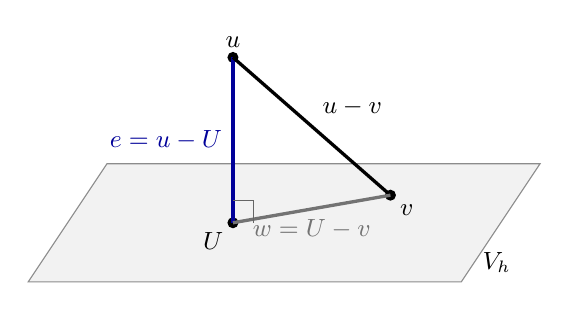
\begin{tikzpicture}[>=Latex,scale=1.0]
  % the subspace as a plane
  \draw[fill=black!5,draw=black!45] (-2.6,-0.75) -- (2.9,-0.75)
        -- (3.9,0.75) -- (-1.6,0.75) -- cycle;
  \node[font=\small] at (3.35,-0.5) {$V_h$};
  % points
  \coordinate (U) at (0,0);
  \coordinate (u) at (0,2.1);
  \coordinate (v) at (2.0,0.35);
  \fill (U) circle (2pt); \node[below left,font=\small]  at (U) {$U$};
  \fill (u) circle (2pt); \node[above,font=\small]       at (u) {$u$};
  \fill (v) circle (2pt); \node[below right,font=\small] at (v) {$v$};
  % the error (perpendicular) and the hypotenuse
  \draw[very thick,blue!60!black] (u) -- (U)
        node[midway,left,font=\small,blue!60!black] {$e=u-U$};
  \draw[very thick] (u) -- (v)
        node[midway,above right,font=\small] {$u-v$};
  \draw[very thick,black!55] (U) -- (v)
        node[midway,below,font=\small,black!55] {$w=U-v$};
  % right-angle mark at U
  \draw[black!60] (0,0.28) -- (0.26,0.28) -- (0.26,0);
\end{tikzpicture}
\par\smallskip
{\small Galerkin orthogonality says the blue leg is perpendicular to the whole
subspace. Every $v\in V_h$ is the far end of a right triangle whose legs are
$e$ and $w$, so the hypotenuse $\norm{u-v}_E$ can never be shorter than
$\norm{e}_E$ --- which is \eqr{eq:pyth}.}
\end{minipage}
\end{center}

\medskip
\textbf{Part 2: the a priori estimate.}
\eqr{eq:opt} holds for \emph{every} $v\in V_h$, so we are free to choose the
most convenient one. Take the nodal interpolant $\pi_h u\in V_h$,
\[
  \pi_h u(x)=\sum_{j=0}^{M}u(x_j)\,\varphi_j(x).
\]

\note{$\pi_h u$ really is in $V_h$: it is continuous piecewise linear by
construction, and it is periodic because $\pi_h u(-\pi)=u(-\pi)=u(\pi)=\pi_h
u(\pi)$. The single nodal value $\xi_0$ at the glued node is assigned $u(x_0)$,
consistently at both ends.}

Assume $u$ is regular enough that $u''\in L^{2}(-\pi,\pi)$. The standard
interpolation estimates for a continuous piecewise linear interpolant are
\begin{equation}\label{eq:interp}
  \norm{u-\pi_h u}_{L^{2}}\le C_{2}\,\norm{h^{2}u''}_{L^{2}},
  \qquad
  \norm{(u-\pi_h u)'}_{L^{2}}\le C_{1}\,\norm{h\,u''}_{L^{2}} .
\end{equation}
Insert them into the energy norm \eqr{eq:enorm} of the interpolation error,
taking $h$ constant and writing $q_{\max}=\max_{[-\pi,\pi]}q$:
\begin{equation}\label{eq:enorminterp}
  \norm{u-\pi_h u}_{E}^{2}
   =\underbrace{\norm{(u-\pi_h u)'}_{L^{2}}^{2}}_{\le\,C_{1}^{2}h^{2}\norm{u''}^{2}}
   +\underbrace{\int_{-\pi}^{\pi}q\,(u-\pi_h u)^{2}\dx}_{\le\,q_{\max}C_{2}^{2}h^{4}\norm{u''}^{2}}
   \;\le\;h^{2}\bigl(C_{1}^{2}+q_{\max}C_{2}^{2}h^{2}\bigr)\norm{u''}_{L^{2}}^{2}.
\end{equation}
Combining \eqr{eq:opt} with $v=\pi_h u$ and \eqr{eq:enorminterp},
\begin{equation}\label{eq:apriori}
  \boxed{\;\norm{u-U}_{E}\;\le\;\norm{u-\pi_h u}_{E}
        \;\le\;C\,h\,\norm{u''}_{L^{2}(-\pi,\pi)},
        \qquad C:=\sqrt{C_{1}^{2}+4\pi^{2}q_{\max}C_{2}^{2}}\;}
\end{equation}
so the CG(1) error in the energy norm is $O(h)$, i.e.\ \textbf{first order}.
Here the residual $h^{2}$ left inside the square root in \eqr{eq:enorminterp}
was removed using $h=2\pi/(M+1)\le2\pi$, so that $C$ depends only on
$q_{\max}$ and the two interpolation constants --- and not on the mesh, as an
\emph{a priori} constant should not.

\note{Two distinct ideas are doing the work, and it is worth separating them.
\eqr{eq:opt} is about the \emph{method}: Galerkin picks the best member of
$V_h$, whatever $V_h$ is. \eqr{eq:interp} is about the \emph{space}: how well
piecewise linears can represent $u$ at all. The method contributes no error of
its own --- the entire $O(h)$ comes from the approximation power of the mesh.
This is the rate to expect from the convergence table in Problem~5.}

\clearpage
% ==================================================================
\section*{Problem 4}

\textbf{Problem.} Prove an \emph{a priori} error estimate in the $L^{2}$-norm.

\subsection*{Solution}

Write $(v,w)=\int_{-\pi}^{\pi}v\,w\dx$ and $\norm{v}=\sqrt{(v,v)}$ for the
$L^{2}$ inner product and norm, and keep $e=u-U$.

The energy estimate \eqr{eq:apriori} is only $O(h)$. To gain a power of $h$ we
use a duality argument: instead of estimating $e$ directly, we feed it as data
into an auxiliary problem.

\medskip
\textbf{Step 1: the dual problem.} Define $\phi$ by the variational problem
\begin{equation}\label{eq:dualvar}
  a(\phi,v)=(e,v)\qquad\forall\,v\in V ,
\end{equation}
which is \eqr{eq:var} with the error $e$ in place of the load $f$. The same
bilinear form $a$ appears on the left because the operator is self-adjoint ---
that is what makes the dual problem the \emph{same} problem.

Taking \eqr{eq:dualvar}, rather than a strong form, as the definition keeps the
logic in order. A unique $\phi\in V$ exists: $a$ is bounded on $V$, coercive by
\eqr{eq:posdef} together with $q_{\min}>0$, and $v\mapsto(e,v)$ is a bounded
linear functional, so Lax--Milgram applies. Regularity then \emph{follows}
instead of being assumed: testing \eqr{eq:dualvar} with
$v\in C^{\infty}_{c}(-\pi,\pi)$ gives $\phi''=q\phi-e$ in the distributional
sense, and the right-hand side lies in $L^{2}$, so $\phi\in H^{2}$. Only now is
the strong form meaningful pointwise,
\begin{equation}\label{eq:dual}
  -\phi''+q(x)\,\phi=e \ \ \text{a.e.\ on }(-\pi,\pi),
  \qquad \phi(-\pi)=\phi(\pi),
  \qquad \phi'(-\pi)=\phi'(\pi),
\end{equation}
the periodicity of $\phi'$ being recovered from \eqr{eq:dualvar} exactly as BC2
was recovered in Problem~1. It is this $H^{2}$ regularity that Step~3 uses when
it differentiates $\phi$ twice.

\medskip
\textbf{Step 2: the chain.} Put $v=e$ in \eqr{eq:dualvar}, use symmetry of $a$,
then subtract $a(e,\pi_h\phi)=0$ --- which is Galerkin orthogonality
\eqr{eq:goa}, legitimate because $\pi_h\phi\in V_h$ --- and finish with the
Cauchy--Schwarz inequality for the inner product $a$:
\begin{equation}\label{eq:chain}
\begin{aligned}
  \norm{e}^{2}
  &=(e,e) \\
  &=a(\phi,e)                       &&\text{by \eqr{eq:dualvar} with }v=e\\
  &=a(e,\phi)                       &&a\text{ is symmetric}\\
  &=a\bigl(e,\ \phi-\pi_h\phi\bigr) &&\text{since }a(e,\pi_h\phi)=0\\
  &\le\norm{e}_{E}\,\norm{\phi-\pi_h\phi}_{E}
                                    &&\text{Cauchy--Schwarz in }a .
\end{aligned}
\end{equation}
By \eqr{eq:enorminterp} applied to $\phi$ instead of $u$,
$\norm{\phi-\pi_h\phi}_{E}\le C\,h\,\norm{\phi''}$, so
\[
  \norm{e}^{2}\;\le\;C\,h\,\norm{e}_{E}\,\norm{\phi''} .
\]
It remains to trade $\norm{\phi''}$ for $\norm{e}$.

\medskip
\textbf{Step 3: stability of the dual problem.}
First bound $\phi$ itself. Put $v=\phi$ in \eqr{eq:dualvar} and write
$q_{\min}=\min_{[-\pi,\pi]}q>0$:
\[
  q_{\min}\norm{\phi}^{2}
  \;\le\;\int_{-\pi}^{\pi}\Bigl[(\phi')^{2}+q\,\phi^{2}\Bigr]\dx
  \;=\;\norm{\phi}_{E}^{2}\;=\;(e,\phi)\;\le\;\norm{e}\,\norm{\phi},
\]
so that
\begin{equation}\label{eq:phibound}
  \norm{\phi}\;\le\;\frac{1}{q_{\min}}\,\norm{e} .
\end{equation}
Now read $\phi''$ off the differential equation \eqr{eq:dual} itself,
$\phi''=q\phi-e$, and use \eqr{eq:phibound}:
\begin{equation}\label{eq:stab}
  \norm{\phi''}\;\le\;q_{\max}\norm{\phi}+\norm{e}
  \;\le\;\underbrace{\Bigl(1+\frac{q_{\max}}{q_{\min}}\Bigr)}_{=:\,C_{S}}\norm{e} .
\end{equation}

\note{This is the step where the periodic problem genuinely differs from the
Dirichlet one. In Lecture~8 the stability constant came from the
\textbf{Poincar\'e inequality}, which bounds $\norm{\phi}$ by $\norm{\phi'}$.
That inequality is \emph{false} on the periodic space \eqr{eq:space}: a nonzero
constant has $\phi'\equiv0$ but $\norm{\phi}\neq0$. With no boundary condition
pinning the function down, the zeroth-order term $q$ is what supplies
stability instead --- which is why $q_{\min}>0$ appears in
\eqr{eq:phibound}. It is the same role $q>0$ played in \eqr{eq:posdef} and in
the nonsingularity of $\bm{A}$.}

\medskip
\textbf{Step 4: combine.} Substituting \eqr{eq:stab} into the result of
Step~2,
\[
  \norm{e}^{2}\;\le\;C\,C_{S}\,h\,\norm{e}_{E}\,\norm{e}
  \qquad\Longrightarrow\qquad
  \norm{e}\;\le\;C\,C_{S}\,h\,\norm{e}_{E},
\]
after cancelling one factor $\norm{e}$ (if $\norm{e}=0$ there is nothing to
prove). Finally insert the energy estimate \eqr{eq:apriori}:
\begin{equation}\label{eq:l2}
  \boxed{\;\norm{u-U}_{L^{2}(-\pi,\pi)}\;\le\;\widetilde{C}\,h^{2}\,
         \norm{u''}_{L^{2}(-\pi,\pi)},
         \qquad \widetilde{C}=C^{2}C_{S}\;}
\end{equation}
so the CG(1) error in $L^{2}$ is $O(h^{2})$, i.e.\ \textbf{second order} ---
one power of $h$ better than the energy norm.

\note{Where the extra power came from: \eqr{eq:chain} pairs the error against
the \emph{interpolation error of the dual solution} rather than against itself,
and interpolation costs one power of $h$. The duality step is what converts
``$e$ is small in energy'' into ``$e$ is small in $L^{2}$''. These are the two
rates, $O(h)$ and $O(h^{2})$, that the convergence table in Problem~5 has to
reproduce.}

\clearpage
% ==================================================================
\section*{Problem 5}

\textbf{Problem.} Implement CG(1) numerically on a uniform mesh with
\[
  q(x)=3-\sin(x)-\sin(2x)-\cos(x),\quad
  f(x)=2e^{\sin(x)}e^{\cos(x)},\quad
  u(x)=e^{\sin(x)}e^{\cos(x)},
\]
and determine the convergence rate in both the energy norm and the $L^{2}$-norm
by a convergence table with $M=24,49,99,199,399,799$.

\subsection*{Solution}

Code: \texttt{hw2\_p5\_cg1.py} (Python, \texttt{numpy}/\texttt{scipy}).

\medskip
\textbf{Verification of the data.} Before solving anything the script checks
that the stated $u$, $q$, $f$ really are consistent. With
$u=e^{\sin x+\cos x}$,
\[
  u'=u\,(\cos x-\sin x),\qquad
  u''=u\bigl[(\cos x-\sin x)^{2}-(\sin x+\cos x)\bigr],
\]
and since $(\cos x-\sin x)^{2}=1-\sin 2x$,
\[
  -u''+q\,u
   =u\bigl[-1+\sin 2x+\sin x+\cos x+3-\sin x-\sin 2x-\cos x\bigr]=2u=f .\quad\checkmark
\]
Numerically $\max|{-u''}+qu-f|=2.7\times10^{-15}$, and the periodicity defect
$|u(-\pi)-u(\pi)|+|u'(-\pi)-u'(\pi)|=3.3\times10^{-16}$, so $u$ satisfies
\eqr{eq:ode} including both boundary conditions.

\medskip
\textbf{Implementation.} Following Problem~2: $N=M+1$ unknowns and $N$
elements, $h=2\pi/N$. On the reference element $[0,1]$ with
$N_{0}(\xi)=1-\xi$, $N_{1}(\xi)=\xi$, the element contributions to
\eqr{eq:entries} are
\begin{equation}\label{eq:elem}
  \bm{K}^{e}=\frac{1}{h}\begin{bmatrix}1&-1\\-1&1\end{bmatrix},
  \qquad
  M^{e}_{ab}=\int_{I_{e}}q\,N_{a}N_{b}\dx ,
  \qquad
  b^{e}_{a}=\int_{I_{e}}f\,N_{a}\dx .
\end{equation}
$\bm{K}^{e}$ is exact. Because $q$ and $f$ are not polynomials, $M^{e}$ and
$b^{e}$ are evaluated with $6$-point Gauss--Legendre quadrature per element,
which is far more accurate than the $O(h^{2})$ discretisation error and so does
not pollute the observed rates.

The \emph{only} periodic-specific line in the whole assembly is the
local-to-global map:
\begin{equation}\label{eq:wrap}
  \text{element }e\ \longmapsto\ \text{nodes }
  \bigl(e,\ (e+1)\bmod N\bigr),\qquad e=0,1,\dots,N-1 ,
\end{equation}
(the code indexes elements from $0$, so element $e$ here is the element called
$I_{e+1}$ in \eqr{eq:mesh}), where the $\bmod N$ sends the last element's right node back to node~$0$. That
single modulus is what produces the corner entries $A_{0,M}=A_{M,0}$ predicted
in Problem~2 --- no rows or columns are deleted, unlike the Dirichlet case.

The system is solved with \texttt{scipy.sparse.linalg.cg} (tolerance
$10^{-13}$), legitimate because $\bm{A}$ is symmetric positive definite by
Problem~2. Both error norms are computed element by element with the same Gauss
rule, using $u'$ analytically and $U'$ constant on each element.

\medskip
\textbf{Convergence table.} The observed rate between two consecutive meshes is
\begin{equation}\label{eq:rate}
  r_{k}=\frac{\ln\bigl(E_{k-1}/E_{k}\bigr)}{\ln\bigl(h_{k-1}/h_{k}\bigr)} .
\end{equation}

\begin{center}
\begin{tabular}{rccccc}
\toprule
$M$ & $h$ & $\|u-U\|_{L^2}$ & rate & $\|u-U\|_E$ & rate\\
\midrule
24 & 2.5133e-01 & 2.7134e-02 & --- & 4.1346e-01 & ---\\
49 & 1.2566e-01 & 6.7860e-03 & 2.00 & 2.0691e-01 & 1.00\\
99 & 6.2832e-02 & 1.6967e-03 & 2.00 & 1.0348e-01 & 1.00\\
199 & 3.1416e-02 & 4.2418e-04 & 2.00 & 5.1743e-02 & 1.00\\
399 & 1.5708e-02 & 1.0605e-04 & 2.00 & 2.5872e-02 & 1.00\\
799 & 7.8540e-03 & 2.6511e-05 & 2.00 & 1.2936e-02 & 1.00\\
\bottomrule
\end{tabular}

\end{center}

\medskip
\textbf{Conclusion.} The observed rates are
\[
  \norm{u-U}_{E}=O(h^{1.00}),
  \qquad
  \norm{u-U}_{L^{2}}=O(h^{2.00}),
\]
which is exactly the theory: first order in the energy norm from
\eqr{eq:apriori}, and second order in $L^{2}$ from \eqr{eq:l2}.

\begin{figure}[htbp]
\centering
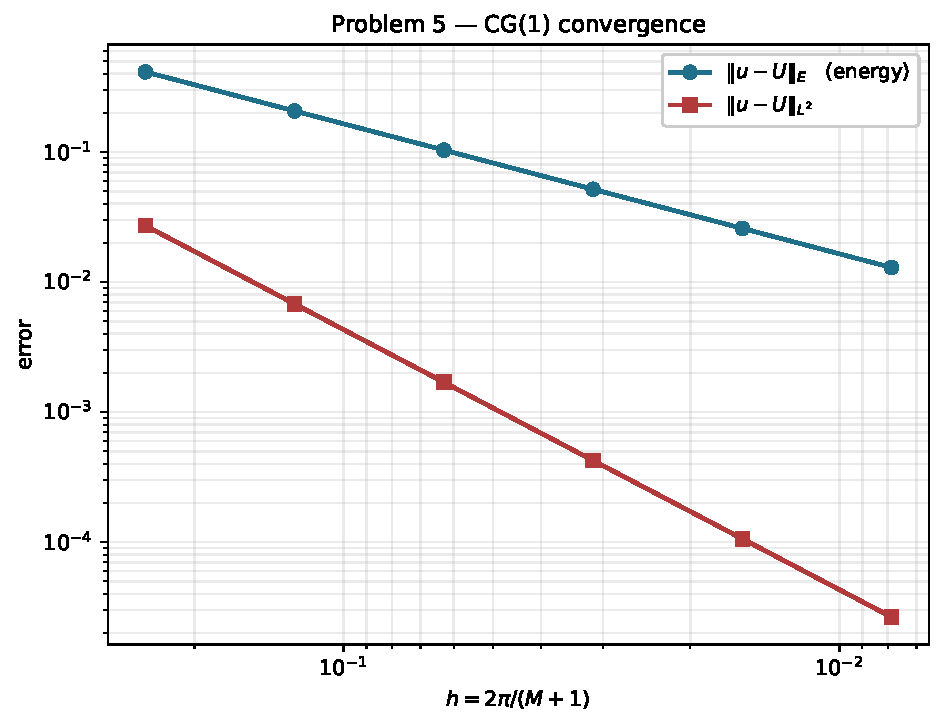
\includegraphics[width=0.86\linewidth]{hw2_p5_convergence.pdf}
\caption*{\small Both error curves are straight on a log--log plot and parallel
to the reference slopes $1$ and $2$ (dashed, offset downward for legibility).}
\end{figure}

\clearpage
\begin{figure}[htbp]
\centering
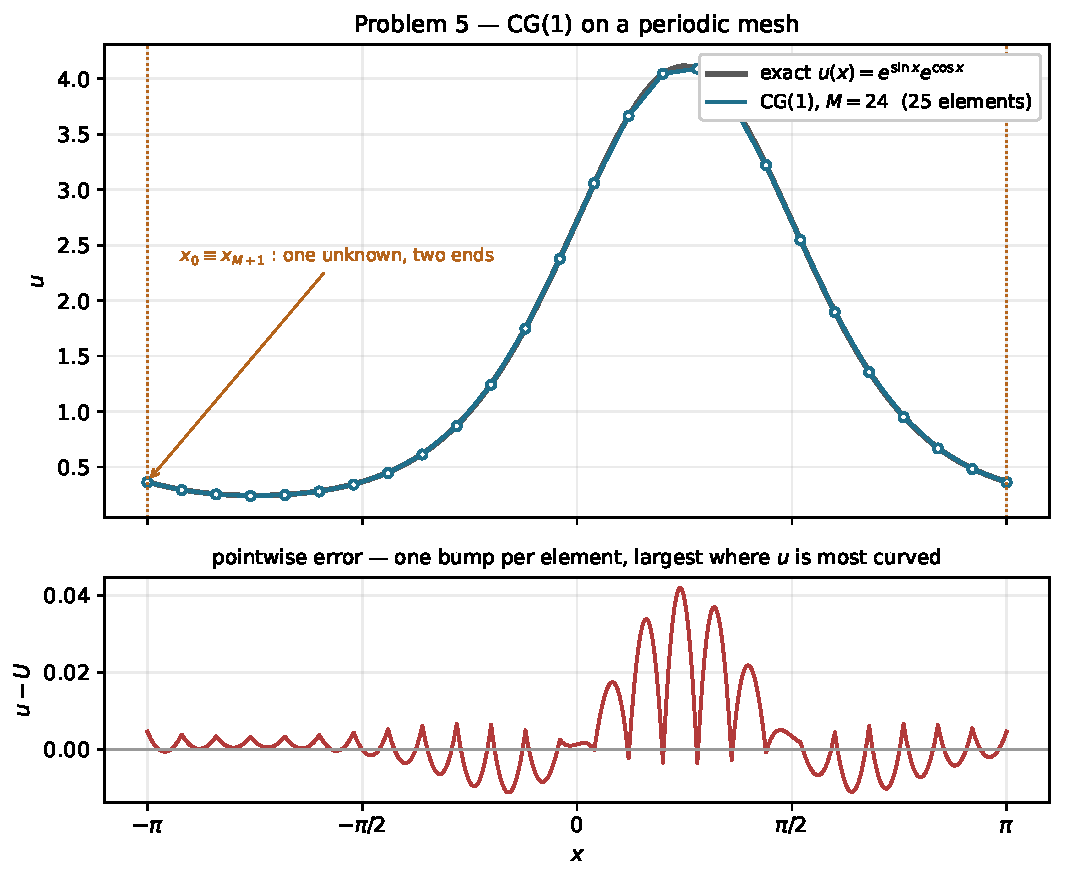
\includegraphics[width=0.94\linewidth]{hw2_p5_solution.pdf}
\caption*{\small \textbf{Top:} exact solution and the CG(1) solution at $M=24$;
the circles are the $25$ nodes. The dotted lines at $x=\pm\pi$ mark the
\emph{same} point of the domain --- one unknown $\xi_{0}$ serving both ends,
which is the wrap-around basis function \eqr{eq:hat0} at work.
\textbf{Bottom:} the pointwise error.}
\end{figure}

\note{The lower panel is where the structure shows: one bump per element,
largest near $x\approx\pi/4$ where $u$ is most strongly curved --- the factor
$\norm{u''}$ of \eqr{eq:apriori} visible directly.

It is worth \emph{measuring} rather than assuming that the error vanishes at the
nodes, because it does not. The script prints a nodal-error column:
$\max_j\bigl|u(x_j)-U_j\bigr|=6.6\times10^{-3}$ at $M=24$, which is
$0.245\,\norm{u-U}_{L^{2}}$, and that ratio stays fixed under refinement --- the
nodal error decays at the same $O(h^{2})$ rate as everything else, it is simply
smaller. CG(1) \emph{is} nodally exact for the pure problem $-u''=f$, but the
zeroth-order term $q\,u$ destroys that property; the mechanism is explained in
the closing note of Problem~7, where the contrast is measured.}

\clearpage
% ==================================================================
\section*{Problem 6}

\textbf{Problem.} Implement the CG(2) method (piecewise quadratic polynomials)
as discussed in class for
\[
  -u''=f(x)\ \text{ on }(0,1),\qquad u(0)=u(1)=0 .
\]

\subsection*{Solution}

Code: \texttt{hw2\_p67\_cg2.py}.

\medskip
\textbf{Variational setting.} The derivation of Problem~1 carries over with
$q\equiv0$ and periodicity replaced by Dirichlet conditions, and the optimality
argument \eqr{eq:opt} of Problem~3 then applies verbatim, since it uses only
Galerkin orthogonality and the fact that $a$ is an inner product. Two things do
\emph{not} carry over: Problem~1's definiteness step used $q>0$ and must be
replaced (see the note below), and the \emph{rate} in \eqr{eq:apriori} was for
piecewise linears, so it is the CG(2) estimates of Lecture~10 that apply here.
The space is
\[
  V=\Bigl\{\,v:\ \int_0^1\bigl(v^{2}+(v')^{2}\bigr)\dx<\infty,
     \ \ v(0)=v(1)=0\,\Bigr\},
\]
and multiplying $-u''=f$ by $v\in V$ and integrating by parts once kills the
boundary term because $v$ vanishes at \emph{both} ends --- here both conditions
are essential, and there is no natural one. So: find $u\in V$ with
\[
  a(u,v)=\int_0^1 u'v'\dx=\int_0^1 f\,v\dx\qquad\forall\,v\in V,
  \qquad\text{hence}\qquad
  \norm{v}_{E}^{2}=\int_0^1(v')^{2}\dx .
\]
Taking $V_h\subset V$ and subtracting exactly as in \eqr{eq:go} gives Galerkin
orthogonality $a(u-U,v)=0$ for all $v\in V_h$, so the optimality result
\eqr{eq:opt} of Problem~3 applies verbatim here too.

\note{$\norm{\cdot}_{E}$ really is a norm on this $V$ even though there is no
$q$ term: $v'\equiv0$ forces $v$ constant, and $v(0)=0$ then forces $v\equiv0$.
On $H^{1}(0,1)$ \emph{without} the boundary conditions it would be only a
seminorm. This is the Dirichlet counterpart of the remark closing Problem~1 ---
there it was $q>0$ that eliminated the constants, here it is the boundary
condition.}

\medskip
\textbf{Mesh and numbering.} With $h=1/(M+1)$ there are $M+1$ elements and, as
in Lecture~10, a submesh carrying one midside node per element. Index every
node by a half-integer:
\begin{equation}\label{eq:p6num}
  x_{k/2}=\tfrac{k h}{2},\quad k=0,1,\dots,2M+2 :
  \qquad
  \text{$k$ even}\ \Rightarrow\ \text{vertex},
  \qquad
  \text{$k$ odd}\ \Rightarrow\ \text{midside} .
\end{equation}
That is $2M+3$ nodes; the two Dirichlet ends $k=0$ and $k=2M+2$ are eliminated,
leaving \textbf{$2M+1$ unknowns} --- the size Lecture~10 predicts.

\medskip
\textbf{Basis.} On the reference element $[0,1]$ the three Lagrange quadratics
are
\begin{equation}\label{eq:p6shape}
  N_{0}(\xi)=2\bigl(\xi-\tfrac12\bigr)(\xi-1),
  \qquad
  N_{1}(\xi)=4\xi(1-\xi),
  \qquad
  N_{2}(\xi)=2\xi\bigl(\xi-\tfrac12\bigr),
\end{equation}
taking the value $1$ at $\xi=0,\ \tfrac12,\ 1$ respectively and $0$ at the other
two. These are the three Lagrange polynomials of Lecture~10 written on a single
element.

\medskip
\textbf{Element stiffness.} With $\mathrm{d}N_{a}/\mathrm{d}x=
h^{-1}\mathrm{d}N_{a}/\mathrm{d}\xi$,
\[
  K^{e}_{ab}=\frac1h\int_{0}^{1}
    \frac{\mathrm{d}N_{a}}{\mathrm{d}\xi}\frac{\mathrm{d}N_{b}}{\mathrm{d}\xi}
    \,\mathrm{d}\xi ,
  \qquad
  \frac{\mathrm{d}N_{0}}{\mathrm{d}\xi}=4\xi-3,\ \
  \frac{\mathrm{d}N_{1}}{\mathrm{d}\xi}=4-8\xi,\ \
  \frac{\mathrm{d}N_{2}}{\mathrm{d}\xi}=4\xi-1,
\]
which integrates exactly to
\begin{equation}\label{eq:p6Ke}
  \bm{K}^{e}=\frac{1}{3h}
  \begin{bmatrix}
     7 & -8 &  1\\
    -8 & 16 & -8\\
     1 & -8 &  7
  \end{bmatrix}
  \qquad\text{(ordering: vertex, midside, vertex).}
\end{equation}
The load $b^{e}_{a}=\int_{I_{e}}f\,N_{a}\dx$ is evaluated with $8$-point
Gauss--Legendre quadrature, since $f$ is not a polynomial.

\note{Lecture~10 instead replaces $f$ by its interpolant $\widetilde\Pi_h f$,
giving $f_i=\tfrac{h}{15}\bigl[f+8f+f\bigr]$ on the midside rows and
$\tfrac{h}{30}\bigl[-f+2f+8f+2f-f\bigr]$ on the vertex rows. That choice does
not change the \emph{asymptotic} rates. Implementing it (see
\texttt{interp\_load\_compare()} in the script) and differencing the two
discrete solutions gives
$\norm{U_{\mathrm{interp}}-U_{\mathrm{Gauss}}}=O(h^{4})$ in both norms:
measured rates $3.97,3.99,4.00,4.00,4.00$ in $L^{2}$ and
$4.01,4.00,4.00,4.00,4.00$ in the energy norm --- two orders below the
$O(h^{2})$ energy error and one below the $O(h^{3})$ $L^{2}$ error.

It is not, however, invisible in the table \emph{as printed}, because the table
starts before the two have separated. With the interpolated load the $L^{2}$
entry at $M=24$ moves from $1.11\times10^{-3}$ to $1.14\times10^{-3}$, and the
first printed $L^{2}$ rate moves from $2.99$ to $3.02$. From $M=99$ onwards the
$L^{2}$ column agrees to three digits, and the energy column agrees to three
digits at every $M$.

So there are two reasons to prefer accurate quadrature here, neither of them the
asymptotic rate: it keeps the coarse rows clean, and it preserves the
machine-exact vertex values discussed at the end of Problem~7 --- with the
interpolated load those degrade to $O(h^{4})$ ($3.2\times10^{-4}$ at $M=24$,
rates $3.97$--$4.02$; the $3.65$ printed for the finest mesh is the roundoff
floor, since $\operatorname{cond}(\bm{A})=O(h^{-2})$ puts solver noise at
$\sim10^{-9}$ there).}

\medskip
\textbf{Verification against the lecture.} Assembling \eqr{eq:p6Ke} over the
elements and striking out the two Dirichlet rows and columns, the code prints
$3h\bm{A}$ for $M=4$ (a $9\times9$ system):
\begin{equation}\label{eq:p6assembled}
  3h\,\bm{A}=
  \setlength{\arraycolsep}{3.2pt}
  \renewcommand{\arraystretch}{0.92}
  \begin{bmatrix}
   16 & -8 &    &    &    &    &    &    &   \\
   -8 & 14 & -8 &  1 &    &    &    &    &   \\
      & -8 & 16 & -8 &    &    &    &    &   \\
      &  1 & -8 & 14 & -8 &  1 &    &    &   \\
      &    &    & -8 & 16 & -8 &    &    &   \\
      &    &    &  1 & -8 & 14 & -8 &  1 &   \\
      &    &    &    &    & -8 & 16 & -8 &   \\
      &    &    &    &    &  1 & -8 & 14 & -8\\
      &    &    &    &    &    &    & -8 & 16
  \end{bmatrix}
\end{equation}
This reproduces Lecture~10 exactly: $16/3h$ on the midside diagonal, $14/3h$ on
the vertex diagonal, $-8/3h$ on the first off-diagonal and $1/3h$ two places out
from a vertex row. The matrix is symmetric positive definite, which is what
\texttt{cg} requires. Its pattern is \emph{pentadiagonal} rather than
tridiagonal: raising the polynomial degree widens the band, because a vertex row
now reaches the vertex two places away through the shared midside. That is a
separate effect from the wrap-around corners of Problem~2, which came from
periodicity and not from the degree --- the CG(1) matrix there is not
tridiagonal either, for a different reason.

% ==================================================================
\clearpage
\section*{Problem 7}

\textbf{Problem.} Apply the method to
\[
  u(x)=e^{1-\cos(2\pi x)-\sin(2\pi x)}-1,\qquad
  f(x)=4\pi^{2}e^{1-\cos(2\pi x)-\sin(2\pi x)}
       \Bigl[\sin(4\pi x)-\cos(2\pi x)-\sin(2\pi x)-1\Bigr],
\]
and determine the convergence rate in both norms for
$M=24,49,99,199,399,799$.

\subsection*{Solution}

\textbf{Verification of the data.} Write $g(x)=1-\cos(2\pi x)-\sin(2\pi x)$, so
$u=e^{g}-1$ and
\[
  g'=2\pi\bigl(\sin 2\pi x-\cos 2\pi x\bigr),\qquad
  g''=4\pi^{2}\bigl(\cos 2\pi x+\sin 2\pi x\bigr),\qquad
  (g')^{2}=4\pi^{2}\bigl(1-\sin 4\pi x\bigr).
\]
Then $u''=e^{g}\bigl[(g')^{2}+g''\bigr]$, so
\begin{equation}\label{eq:p7data}
  -u''=4\pi^{2}e^{g}\Bigl[\sin 4\pi x-\cos 2\pi x-\sin 2\pi x-1\Bigr]=f .
  \quad\checkmark
\end{equation}
Also $u(0)=u(1)=e^{0}-1=0$, so both boundary conditions hold. Numerically
$\max|{-u''}-f|=3.4\times10^{-13}$ and $|u(0)|+|u(1)|=2.2\times10^{-16}$.

\medskip
\textbf{Convergence table.}
\begin{center}
\begin{tabular}{rccccc}
\toprule
$M$ & $h$ & $\|u-U\|_{L^2}$ & rate & $\|u-U\|_E$ & rate\\
\midrule
24 & 4.0000e-02 & 1.1132e-03 & --- & 1.8041e-01 & ---\\
49 & 2.0000e-02 & 1.3975e-04 & 2.99 & 4.5288e-02 & 1.99\\
99 & 1.0000e-02 & 1.7488e-05 & 3.00 & 1.1334e-02 & 2.00\\
199 & 5.0000e-03 & 2.1866e-06 & 3.00 & 2.8341e-03 & 2.00\\
399 & 2.5000e-03 & 2.7334e-07 & 3.00 & 7.0857e-04 & 2.00\\
799 & 1.2500e-03 & 3.4168e-08 & 3.00 & 1.7715e-04 & 2.00\\
\bottomrule
\end{tabular}

\end{center}

\textbf{Conclusion.} The observed rates are
\[
  \norm{u-U}_{E}=O(h^{2.00}),
  \qquad
  \norm{u-U}_{L^{2}}=O(h^{3.00}),
\]
matching the CG(2) estimates quoted in Lecture~10,
$\norm{u-U}_{E}\le c\norm{h^{2}u'''}$ and $\norm{u-U}\le c\norm{h^{3}u'''}$.
Each extra polynomial degree buys one power of $h$ in both norms, and $L^{2}$
stays one order ahead of the energy norm. The \emph{structure} of the duality
argument of Problem~4 is what delivers that extra order, and it does not care
what degree the elements are --- but its stability step does not carry over
unchanged: with $q\equiv0$ the bound \eqr{eq:phibound} is vacuous and
$C_{S}=1+q_{\max}/q_{\min}$ is undefined. Here the dual problem is simply
$-\phi''=e$ with $\phi(0)=\phi(1)=0$, so $\norm{\phi''}=\norm{e}$ is immediate
and $C_{S}=1$: the \emph{stability} step needs neither $q_{\min}$ nor a
Poincar\'e inequality.

\note{Poincar\'e does not disappear from the Dirichlet problem altogether, and
it is worth saying where it goes. With $q\equiv0$ it is what makes $a$ coercive
on $V$ at all --- $\int(v')^{2}\ge c\norm{v}_{H^{1}}^{2}$ requires it --- so it
takes over the role that $q_{\min}>0$ played in the existence argument of
Problem~4, Step~1. What it is \emph{not} needed for here is the stability bound,
because $-\phi''=e$ hands over $\phi''$ directly. For a variable coefficient,
$-(a\phi')'=e$, that shortcut is unavailable and Poincar\'e returns to the
stability step as well --- which is the situation of Lecture~8 referred to in
Problem~4.}

\begin{figure}[htbp]
\centering
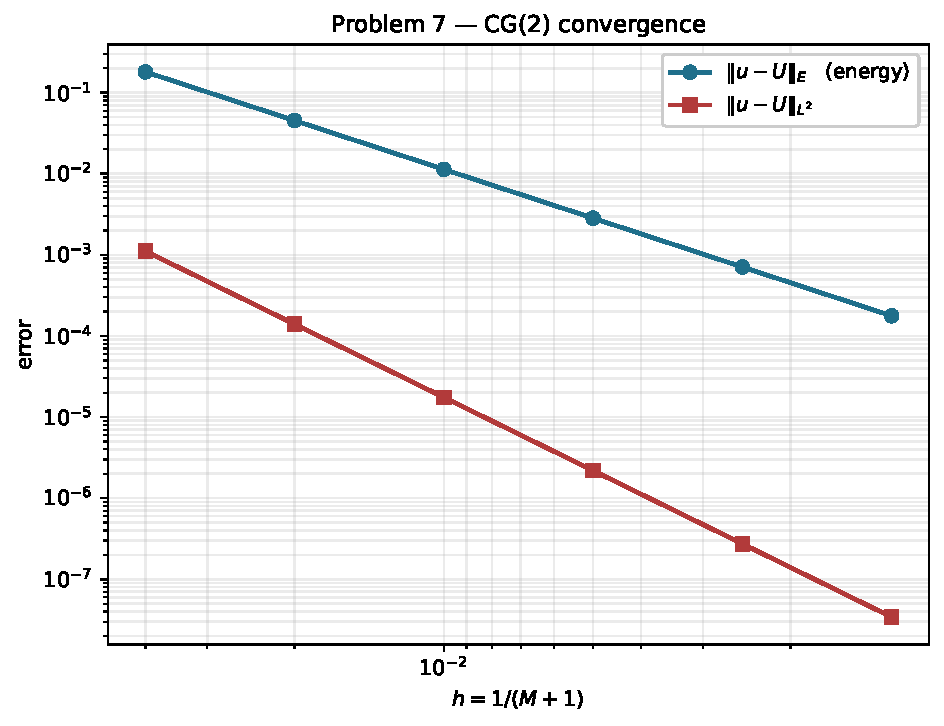
\includegraphics[width=0.86\linewidth]{hw2_p67_convergence.pdf}
\caption*{\small Reference slopes $2$ and $3$ dashed, offset downward for
legibility.}
\end{figure}

\clearpage
\begin{figure}[htbp]
\centering
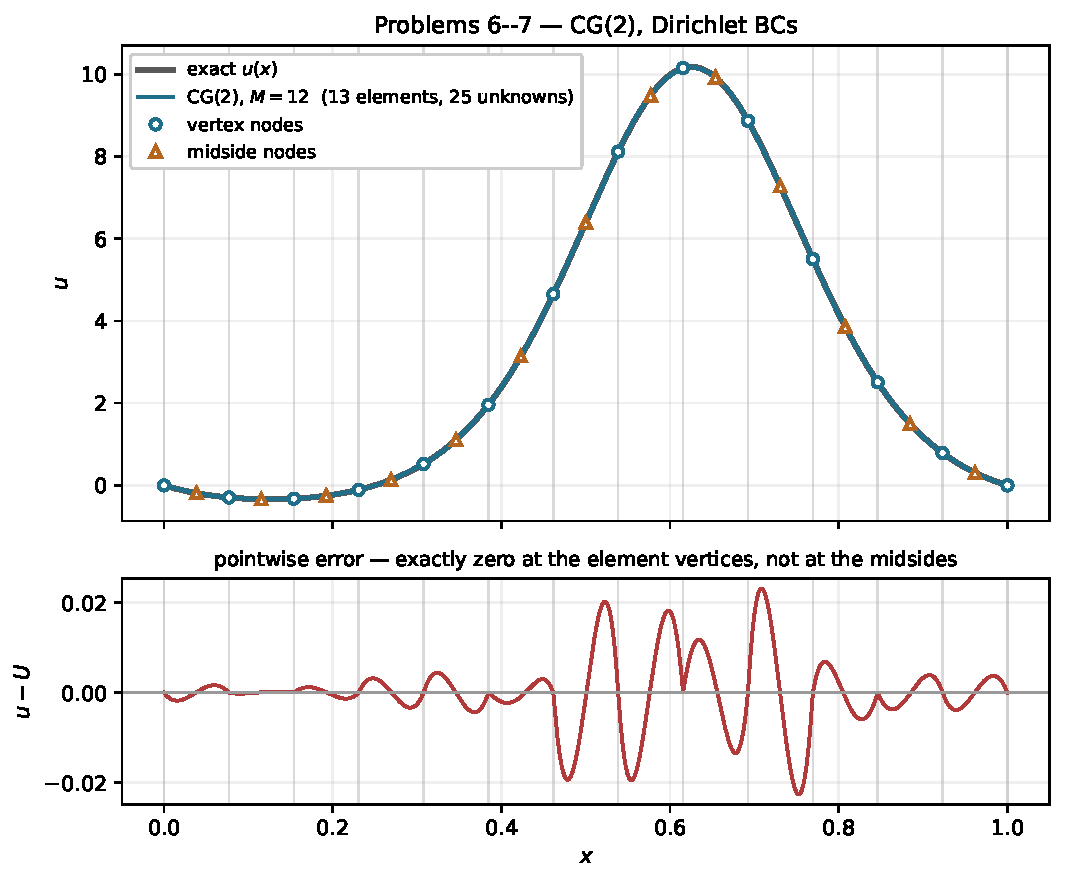
\includegraphics[width=0.94\linewidth]{hw2_p67_solution.pdf}
\caption*{\small \textbf{Top:} exact and CG(2) solutions at $M=12$; circles are
vertex nodes, triangles midside nodes. \textbf{Bottom:} the pointwise error.}
\end{figure}

\note{Here the error \emph{is} exactly zero at the element vertices: the script
prints $\max_j|u(x_j)-U(x_j)|=1.3\times10^{-13}$ at $M=12$, i.e.\ roundoff ---
but \emph{not} at the midsides, where it is $1.9\times10^{-3}$.

\textbf{Why.} It is the Green's function. Let $G(\,\cdot\,;x_j)$ solve
$-G''=\delta(\cdot-x_j)$ with homogeneous Dirichlet ends --- the function
computed in HW1, Problem~1(d). It is piecewise linear with its only kink at
$x_j$, and it satisfies $a(v,G(\,\cdot\,;x_j))=v(x_j)$ for every $v\in V$. If
$x_j$ is a mesh \emph{vertex}, then $G(\,\cdot\,;x_j)$ is linear on every
element, hence $G(\,\cdot\,;x_j)\in V_h$, and therefore
\[
  u(x_j)-U(x_j)=a\bigl(u-U,\ G(\,\cdot\,;x_j)\bigr)=0
\]
by Galerkin orthogonality. Three hypotheses are visible in that one line, and
each one fails somewhere in this homework:
\begin{itemize}\setlength{\itemsep}{1pt}
\item the operator must be $-\mathrm{d}^{2}/\mathrm{d}x^{2}$. With a zeroth-order
  term the Green's function of $-G''+qG=\delta$ is no longer piecewise linear,
  so it leaves $V_h$ --- which is why Problem~5 has no such exactness;
\item the point must be a mesh \emph{vertex}. If $x_j$ is a midside then the
  kink of $G(\,\cdot\,;x_j)$ falls in the \emph{interior} of an element rather
  than at a mesh breakpoint, so $G$ is not a polynomial on that element and
  leaves $V_h$ --- hence the $1.9\times10^{-3}$;
\item the load must be integrated exactly, or $U$ is not the Galerkin solution
  and the orthogonality fails. With Lecture~10's interpolated load the vertex
  error degrades to $O(h^{4})$, as noted in Problem~6.
\end{itemize}
So vertex exactness is a joint property of the operator, the mesh and the
quadrature --- not something the finite element method supplies on its own. It
is also one-dimensional: the argument works only because the Green's function of
a point load is itself a continuous piecewise polynomial. In two dimensions the
Green's function of $-\Delta$ is log-singular and not even in $H^{1}$, so it is
never in $V_h$ and there is no nodal exactness to be had.}

\end{document}
